\documentclass[12pt]{article}\usepackage[]{graphicx}\usepackage[]{color}
%% maxwidth is the original width if it is less than linewidth
%% otherwise use linewidth (to make sure the graphics do not exceed the margin)
\makeatletter
\def\maxwidth{ %
  \ifdim\Gin@nat@width>\linewidth
    \linewidth
  \else
    \Gin@nat@width
  \fi
}
\makeatother

\definecolor{fgcolor}{rgb}{0.345, 0.345, 0.345}
\newcommand{\hlnum}[1]{\textcolor[rgb]{0.686,0.059,0.569}{#1}}%
\newcommand{\hlstr}[1]{\textcolor[rgb]{0.192,0.494,0.8}{#1}}%
\newcommand{\hlcom}[1]{\textcolor[rgb]{0.678,0.584,0.686}{\textit{#1}}}%
\newcommand{\hlopt}[1]{\textcolor[rgb]{0,0,0}{#1}}%
\newcommand{\hlstd}[1]{\textcolor[rgb]{0.345,0.345,0.345}{#1}}%
\newcommand{\hlkwa}[1]{\textcolor[rgb]{0.161,0.373,0.58}{\textbf{#1}}}%
\newcommand{\hlkwb}[1]{\textcolor[rgb]{0.69,0.353,0.396}{#1}}%
\newcommand{\hlkwc}[1]{\textcolor[rgb]{0.333,0.667,0.333}{#1}}%
\newcommand{\hlkwd}[1]{\textcolor[rgb]{0.737,0.353,0.396}{\textbf{#1}}}%
\let\hlipl\hlkwb

\usepackage{framed}
\makeatletter
\newenvironment{kframe}{%
 \def\at@end@of@kframe{}%
 \ifinner\ifhmode%
  \def\at@end@of@kframe{\end{minipage}}%
  \begin{minipage}{\columnwidth}%
 \fi\fi%
 \def\FrameCommand##1{\hskip\@totalleftmargin \hskip-\fboxsep
 \colorbox{shadecolor}{##1}\hskip-\fboxsep
     % There is no \\@totalrightmargin, so:
     \hskip-\linewidth \hskip-\@totalleftmargin \hskip\columnwidth}%
 \MakeFramed {\advance\hsize-\width
   \@totalleftmargin\z@ \linewidth\hsize
   \@setminipage}}%
 {\par\unskip\endMakeFramed%
 \at@end@of@kframe}
\makeatother

\definecolor{shadecolor}{rgb}{.97, .97, .97}
\definecolor{messagecolor}{rgb}{0, 0, 0}
\definecolor{warningcolor}{rgb}{1, 0, 1}
\definecolor{errorcolor}{rgb}{1, 0, 0}
\newenvironment{knitrout}{}{} % an empty environment to be redefined in TeX

\usepackage{alltt}

%% packages
\usepackage{scrtime}  % for \thistime (this package MUST be listed first!)
\usepackage[margin=1in]{geometry} % page layout
\usepackage{amsmath}  % essential for cases environment
\usepackage{amsthm}   % for theorems and proofs
\usepackage{amsfonts} % mathbb
\usepackage{graphics,graphicx}
\usepackage{multirow} % fancy tables
\usepackage{wasysym}  % circle symbols (including half-filled circles)
\usepackage{enumerate}% fancier enumeration (e.g., a,b,c, ...)
%\usepackage{xcolor}
\usepackage{color}

\usepackage{amssymb,latexsym,setspace}
%%\usepackage[colorlinks,linkcolor=blue]{hyperref}
\usepackage[colorlinks=true,allcolors=blue]{hyperref}
\usepackage{xspace}
\usepackage{subfigure}
\usepackage{lineno}
\usepackage{fancyhdr}
\usepackage[english]{babel}  %% for texi2dvi ~ bug
\usepackage[normalem]{ulem}
\usepackage{tikz} % http://www.texample.net/tikz/examples/tikzdevice-demo/
  % N.B. version 0.6.3 of tikzDevice from Rforge is required!!
%% improve figure caption typsetting:  (see ~/tex/caption.pdf for manual)
\usepackage[footnotesize,bf]{caption}
\usepackage{placeins} % \FloatBarrier

%% comments
\newcommand{\de}[1]{{\color{red}{\bfseries DE:} #1}}

%% for solutions to multiple choice questions:
\newcommand{\correct}{{\color{blue}\fbox{\color{red}\checkmark} }}

%% macros
\newcommand{\reals}{\mathbb{R}}
\newcommand{\term}[1]{{\bfseries\slshape #1}}
\newcommand{\Ker}{{\text{Ker}\,}}
\newcommand{\Range}{{\text{Range}\,}}
\newcommand{\diag}{{\text{diag}}}
\newcommand{\alg}{{\text{alg}}}
\newcommand{\geom}{{\text{geom}}}
\newcommand{\norm}[1]{\left\|#1\right\|}
\newcommand{\abs}[1]{\left|#1\right|}
\newcommand{\R}{{\cal R}}
\newcommand{\G}{{\cal G}}
\newcommand{\eps}{\varepsilon}
\newcommand{\B}{\cal B}
\newcommand{\Tinf}{T_\textrm{inf}}
\newcommand{\Shat}{{\hat{S}}}
\newcommand{\Ihat}{{\hat{I}}}
\newcommand{\ie}{\emph{i.e., }}
\newcommand{\eg}{\emph{e.g., }}
\newcommand{\Rlogo}{\protect
\includegraphics[height=2ex,keepaspectratio]{./images/Rlogo.pdf}\xspace}
\newcommand{\XPPAUT}{\texttt{XPPAUT}\xspace}
\newcommand{\etal}{\textit{et al}.\xspace}
\newcommand\emphblue[1]{\emph{\color{blue}#1}}

% citation macros
\newcommand{\citen}[1]{\cite{#1}}

% other macros
\newcommand{\avg}[1]{{\left\langle#1\right\rangle}}
\newcommand{\var}[1]{\textrm{var}\left(#1\right)}
\newcommand{\sem}[1]{\textrm{sem}\left(#1\right)}
\newcommand{\natinf}{{\mathcal I}}
\newcommand{\find}{f_{\textrm{i}}}
\newcommand{\fpop}{f_{\textrm{p}}}
\newcommand{\logit}{\textrm{logit}}
\newcommand{\sign}{\textrm{sign}}
\newcommand{\logistic}{\textrm{logistic}}
\newcommand{\code}[1]{{\tt #1}}
\newcommand{\magcode}[1]{{\tt\color{magenta}#1}}
\newcommand{\redcode}[1]{{\tt\color{red}#1}}
\newcommand{\blackcode}[1]{{\tt\color{black}#1}}

%%%%%%%%%%%%%%%%%%%
%% JOURNAL NAMES %%
%%%%%%%%%%%%%%%%%%%
\def\AJE{{\it American Journal of Epidemiology\/}}
\def\PNAS{PNAS}
\def\JAMA{JAMA}
\def\BMB{{\it Bulletin of Mathematical Biology\/}}

% references
\newcommand{\eref}[1]{Equation~\eqref{E:#1}}
\newcommand{\fref}[1]{Figure~\ref{F:#1}}
\newcommand{\tref}[1]{Table~\ref{T:#1}}
\newcommand{\sref}[1]{\S\ref{S:#1}}
% other macros
\newcommand{{\Reff}}{{\mathcal{R}}_{\rm eff}}
\newcommand{{\Sinit}}{S_{\rm init}}
\newcommand{\supp}{Supplementary Information}
\newcommand{\StoppedHere}{\bigskip\bigskip{\textcolor{red}{\hrule\centerline{\bfseries STOPPED HERE}\hrule}}\bigskip\bigskip}
\newcommand{\colvec}[2]{\begin{pmatrix}#1\\#2\end{pmatrix}}
\newcommand{\diagmat}[3]{\begin{pmatrix}#1&0&0\\0&#2&0\\0&0&#3\end{pmatrix}}

\newcommand{\solution}[1]{{\hfill\break\vspace{-0.5\baselineskip}\break\color{blue}\emph{Solution: }#1}}
\newcommand{\tr}{\text{tr}}

\newcommand{\thickredline}{\bigskip{\color{red}\hrule height 5pt}\bigskip}

%% for assignment 3:
\newtheorem{theorem}{Theorem}
\newtheorem{remark}{Remark}
\newcommand{\openset}{{\mathcal O}}
\newcommand{\C}{{\mathcal C}}

%% underline with smash through:
\newcommand*{\undersmash}[1]{\underline{\smash{#1}}}

%% referring to TeX macros
\newcommand\ttbackslash{{\tt\char`\\}}
\newcommand{\macro}[1]{{\tt\ttbackslash#1}}

%%%%%%%%%%%%%%%%%%%%%%%%%%%%%%%%%%%%%%%%%%%%%%%%%%%%%%%
%% QUESTIONS FOR MATH 4MB/6MB ASSIGNMENT 4.          %%
%% The question texts are used in several documents: %%
%% assignment, solutions, template,                  %%
%% hence it is better to load them from this file.   %%
%%%%%%%%%%%%%%%%%%%%%%%%%%%%%%%%%%%%%%%%%%%%%%%%%%%%%%%

\newcommand{\TSa}{%
You should have received the following data files by e-mail:
\begin{center}
\tt
meas\_uk\_\_lon\_1944-94\_wk.csv\\
meas\_uk\_\_lpl\_1944-94\_wk.csv
\end{center}
These plain text comma-separated-value files list weekly cases of measles (in London and Liverpool, England, from 1944 to 1994).  Depending on which research direction you select, you might receive other files in the same \code{ymdc} (year,month,day,count) format, where the count column might contain cases or deaths, for example.  Write the following \Rlogo functions:
}

\newcommand{\TSai}{%
\magcode{read.ymdc()}.  Read a file in \code{ymdc} format and return a data frame containing these data and including a \code{date} column that has \Rlogo's \magcode{Date} class.  The first (and potentially only) argument to this function should be the \code{filename} of the data file to be read.
}  

\newcommand{\TSaii}{%
\magcode{time.plot()}.  Given a data frame produced using \magcode{read.ymdc()}, display the associated time plot.  The first argument of the function should be the data frame.  Further optional argument(s) should allow the user to smooth the time series with a moving average.  By default, this function should create a new plot but there should be an option to add to an existing plot. Implement this by having a logical \code{add} argument that is false by default (\code{add=FALSE}).  This will allow you to add a smoothed version of the time series on top of the raw data, for example.  The final argument should be the ellipsis (\code{\dots}) so that details such as colour and line style can be passed to the plotting commands used in this function.
}

\newcommand{\TSaiii}{%
\magcode{periodogram()}.  Given a data frame produced using \magcode{read.ymdc()}, display the associated \emph{period   periodogram} (power spectrum as a function of period).  The first argument of the function should be the data frame.  By default, the entire time series should be used, but optional argument(s) should allow the user to specify a time range of interest.  Use \Rlogo's \magcode{spectrum()} function to compute the power spectrum.  Have \code{add} and \code{\dots} arguments as in \magcode{time.plot()}. Note that if \code{v} is a vector containing a time series of interest, you can obtain and plot its \emph{frequency} periodogram as follows.
}

\newcommand{\TSb}{%
Using your functions, make a multi-panel plot that clearly shows the temporal pattern of the time series and how its frequency structure changes over time.  Think carefully about how to make this multi-panel figure as clear as possible for yourselves and your readers.  Describe your figure, explaining what aspects of your figure you feel are puzzling or interesting and may be possible to understand using mechanistic mathematical modelling.  (Repeat this for each of the epidemic time series you are given.)
}

\newcommand{\SEintro}{%
Consider the SI model,
%
\begin{equation}\label{E:SI}
  \frac{dI}{dt} = \beta (N-I) I \,, \qquad I(0)=I_0,
\end{equation}
%
where $\beta$ is the transmission rate, $N$ is the population size and $I(t)$ is the number of infected individuals at time $t$.
}

\newcommand{\SEa}{%
Write an \Rlogo function \magcode{SI.Gillespie()} that uses the Gillespie algorithm to produce a realization of a stochastic process whose mean field dynamics are given by equation \eqref{E:SI} in the limit $N\to\infty$.  Your function should have arguments \code{beta}, \code{N}, \code{I0} and \code{tmax} (the time at which to end the simulation).  You may find it helpful (conceptually) to write equation~\eqref{E:SI} in two-variable form:
  \begin{subequations}
    \begin{align}
      \frac{dS}{dt} &= -\beta S I \,, \qquad S(0)=N-I_0, \\
      \frac{dI}{dt} &= \beta S I \,, \qquad\quad I(0)=I_0.
    \end{align}
  \end{subequations}
Note that there is only one type of event that can occur, so the second part of the Gillespie algorithm (what type of event occurred) is trivial for this model.
}

\long\def\SEb{%
Make a multi-panel plot comparing the deterministic and stochastic dynamics of the SI model for $\beta=1$, $I_0=1$ and $N\in\{32,10^2,10^3,10^4\}$ ($N=32$ is close to $10^{1.5}$).  Each panel should correspond to a different value of $N$ and should show 30 stochastic realizations together with the deterministic solution.

\emph{\underline{Note}:} To make stochastic simulations exactly reproducible use \texttt{\color{magenta}set.seed()}.
}

\newcommand{\Rintro}{%
The natural history of smallpox is shown in \fref{smpxnathist}.  The US Centers for Disease Control and Prevention (CDC) has recently discovered that a group of bioterrorists plans to reintroduce smallpox to the United States.  The CDC has reason to believe that the terrorists are also bioengineers and have successfully altered the virus so that it causes the early rash stage to be twice as long as it was when the virus was last circulating naturally in the 1970s.  Moreover, the existing smallpox vaccine apparently provides no protection against the altered virus.  The CDC wants your opinion on how the alterations to the virus will affect $\R_0$ and the expected final size of an epidemic if the planned attack is successful.
}

\newcommand{\Ra}{%
Construct a compartmental (ODE) smallpox transmission model based on the natural history specified in \fref{smpxnathist}, including vital dynamics but ignoring disease-induced death.
}

\newcommand{\Rb}{%
Use a biological argument to find a formula for $\R_0$.
\label{q:R0biol}
}

\newcommand{\Rc}{%
Calculate $\R_0$ using the next generation matrix approach.  \emph{\underline{Note}:} Your solution should include $\mathcal F$, $\mathcal V$, $F$, $V$, and $FV^{-1}$, in the most human-friendly form you can find.  However, feel free to use symbolic manipulation software such as \texttt{Maple}, {\slshape Mathematica\/} or \href{http://www.sagemath.org/}{sage} to help with the necessary algebra and matrix computations.
}

\newcommand{\Rd}{%
Based on your model, and $\R_0\sim5$ for unaltered smallpox, what can you say about the difference in $\R_0$ that can be expected for the newly engineered virus vs.\ the original virus?  
    %% (\emph{\underline{Note}:} If you make use of other sources of information, such as books or web sites, cite them appropriately.)
}

\newcommand{\qRe}{% \Re is TeX's real part symbol so can't use it
Write a paragraph that you can imagine e-mailing to the CDC, in which you do your best to answer their questions.
    %% It would be good to get them to find a formula for the growth
    %% rate and then explain how to use their model to estimate R0 for
    %% the new virus after the growth rate has been measured
    %% empirically.  But, the growth rate cannot be found analytically
    %% (the characteristic polynomial has degree 5) so the problem
    %% becomes longer than I want to burden them with right now.
}

\newcommand{\smpxnathistfig}{%
%
\begin{figure}[h]
\begin{center}
\scalebox{1}{
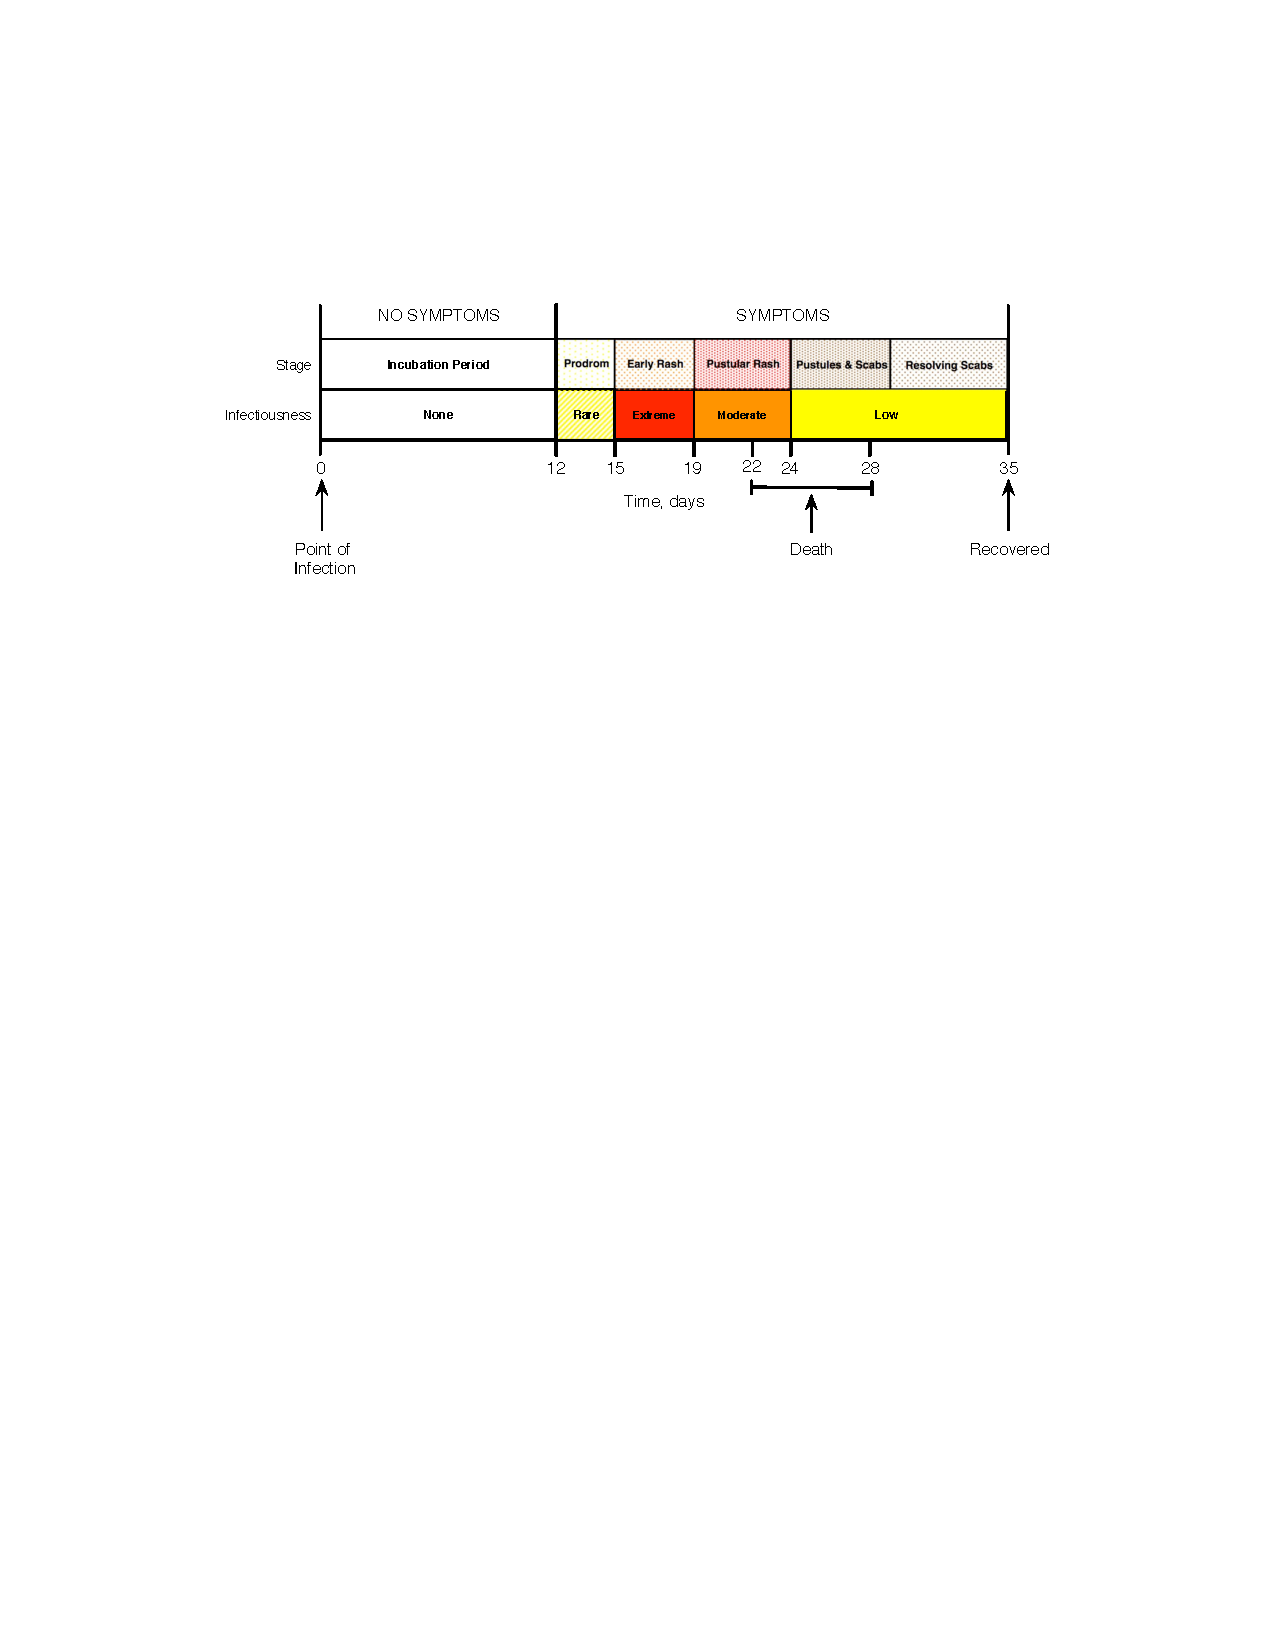
\includegraphics{smpxnathist_p82.pdf}
}
\end{center}
\caption{The natural history of smallpox infection. The prodrom stage begins with fever but the patient is very rarely contagious. Early rash is the most contagious stage, when the rash develops and transforms into bumps. During the pustular rash stage bumps become pustules, which then turn into scabs during the pustules and scabs stage and fall off during the resolving scabs stage. The infected person is contagious until the last scab falls off.  (\emph{This is Figure 3.4 from page 82 of Olga Krylova's 2011 McMaster University PhD thesis.})}
\label{F:smpxnathist}
\end{figure}
%
}

%%\bibliographystyle{vancouver}
%%\bibliography{4mba4_2019}

\newcommand{\BeautifulSolution}{{\color{blue}\begin{proof}{\color{magenta}\dots beautifully clear and concise text to be inserted here\dots}\end{proof}}}
%% FANCY HEADER AND FOOTER STUFF %%
\usepackage{fancyhdr,lastpage}
\pagestyle{fancy}
\fancyhf{} % clear all header and footer parameters
%%%\lhead{Student Name: \theblank{4cm}}
%%%\chead{}
%%%\rhead{Student Number: \theblank{3cm}}
%%%\lfoot{\small\bfseries\ifnum\thepage<\pageref{LastPage}{CONTINUED\\on next page}\else{LAST PAGE}\fi}
\lfoot{}
\cfoot{{\small\bfseries Page \thepage\ of \pageref{LastPage}}}
\rfoot{}
\renewcommand\headrulewidth{0pt} % Removes funny header line
%%%%%%%%%%%%%%%%%%%%%%%%%%%%%%%%%%%
\IfFileExists{upquote.sty}{\usepackage{upquote}}{}
\begin{document}
%Title
\begin{center}
{\bf Mathematics 4MB3/6MB3 Mathematical Biology\\
\smallskip
\url{http://www.math.mcmaster.ca/earn/4MB3}\\
\smallskip
2019 ASSIGNMENT 4}\\
\medskip
\underline{\emph{Group Name}}: \texttt{{\color{blue}The Plague Doctors}}\\
\medskip
\underline{\emph{Group Members}}: {\color{blue}Sid Reed, Daniel Segura, Jessa Mallare, Aref Jadda}
\end{center}

%due date
\bigskip
\noindent
This assignment is {\bfseries\color{red} due in class} on \textcolor{red}{\bf Wednesday March 13 2019 at 10:30am}.
\bigskip
%Answers
\begin{enumerate}
    \item %TSintro
    \begin{enumerate}[(a)]
        \item \TSa
        \begin{enumerate}[(i)]
            \item

% !Rnw root = main.Rnw
\begin{knitrout}
\definecolor{shadecolor}{rgb}{0.969, 0.969, 0.969}\color{fgcolor}\begin{kframe}
\begin{verbatim}
## [1] "First 5 rows of the dataframe"
##   year month day cases       date
## 1 1944     1   7    82 1944-01-07
## 2 1944     1  14    98 1944-01-14
## 3 1944     1  21   118 1944-01-21
## 4 1944     1  28   153 1944-01-28
## 5 1944     2   4   206 1944-02-04
## 6 1944     2  11   217 1944-02-11
\end{verbatim}
\end{kframe}
\end{knitrout}

            \item

% !Rnw root = main.Rnw
\begin{knitrout}
\definecolor{shadecolor}{rgb}{0.969, 0.969, 0.969}\color{fgcolor}\begin{kframe}
\begin{verbatim}
## [1] "smoothing with moving average, a = 10"
\end{verbatim}
\end{kframe}
\includegraphics[width=\maxwidth]{figure/1aii-1} 

\end{knitrout}
            \item

% !Rnw root = main.Rnw
\begin{knitrout}
\definecolor{shadecolor}{rgb}{0.969, 0.969, 0.969}\color{fgcolor}\begin{kframe}
\begin{verbatim}
## [1] "Using pgram estimation method"
\end{verbatim}
\end{kframe}
\includegraphics[width=\maxwidth]{figure/1aiii-1} 

\end{knitrout}


        \end{enumerate}
        \item \TSb

% !Rnw root = main.Rnw
\begin{knitrout}
\definecolor{shadecolor}{rgb}{0.969, 0.969, 0.969}\color{fgcolor}\begin{kframe}
\begin{verbatim}
## [1] "smoothing with moving average, a = 30"
\end{verbatim}
\end{kframe}
\includegraphics[width=\maxwidth]{figure/1b-1} 
\begin{kframe}\begin{verbatim}
## [1] "Using lag k = 1100"
\end{verbatim}
\end{kframe}
\includegraphics[width=\maxwidth]{figure/1b-2} 
\begin{kframe}\begin{verbatim}
## [1] "smoothing with moving average, a = 30"
\end{verbatim}
\end{kframe}
\includegraphics[width=\maxwidth]{figure/1b-3} 
\begin{kframe}\begin{verbatim}
## [1] "Using lag k = 1100"
\end{verbatim}
\end{kframe}
\includegraphics[width=\maxwidth]{figure/1b-4} 

\end{knitrout}
    \end{enumerate}
    \item \SEintro
    \begin{enumerate}[(a)]
        \item

% !Rnw root = main.Rnw
\begin{knitrout}
\definecolor{shadecolor}{rgb}{0.969, 0.969, 0.969}\color{fgcolor}\begin{kframe}
\begin{alltt}
\hlkwd{source}\hlstd{(}\hlstr{'gillespie.R'}\hlstd{)}
\hlcom{#simulation vars}
\hlstd{beta} \hlkwb{=} \hlnum{1}
\hlstd{N} \hlkwb{=} \hlnum{100}
\hlstd{I0} \hlkwb{=} \hlnum{1}
\hlstd{tmax} \hlkwb{=} \hlnum{50}
\hlstd{realizations} \hlkwb{=} \hlnum{30}
\hlstd{result} \hlkwb{<-} \hlkwd{SI.Gillespie}\hlstd{(beta,N,I0,tmax)}
\hlkwd{plot}\hlstd{(result[[}\hlnum{1}\hlstd{]], result[[}\hlnum{2}\hlstd{]],} \hlkwc{col}\hlstd{=}\hlstr{"green"}\hlstd{,} \hlkwc{type}\hlstd{=}\hlstr{"l"}\hlstd{,} \hlkwc{xlab}\hlstd{=}\hlstr{"Time (t)"}\hlstd{,}
     \hlkwc{ylab}\hlstd{=}\hlstr{"Incidence (I(t))"}\hlstd{,} \hlkwc{main}\hlstd{=}\hlkwd{paste}\hlstd{(}\hlstr{"N ="}\hlstd{,N))}
\end{alltt}
\end{kframe}
\includegraphics[width=\maxwidth]{figure/singlegillespie-1} 

\end{knitrout}
        \item

% !Rnw root = main.Rnw
\begin{knitrout}
\definecolor{shadecolor}{rgb}{0.969, 0.969, 0.969}\color{fgcolor}\begin{kframe}
\begin{alltt}
\hlkwd{source}\hlstd{(}\hlstr{'gillespie.R'}\hlstd{)}
\hlcom{#simulation vars}
\hlstd{beta} \hlkwb{=} \hlnum{1}
\hlstd{ns} \hlkwb{=} \hlkwd{c}\hlstd{(}\hlnum{32}\hlstd{,}\hlnum{100}\hlstd{,}\hlnum{1000}\hlstd{,}\hlnum{10000}\hlstd{)}
\hlstd{I0} \hlkwb{=} \hlnum{1}
\hlstd{tmax} \hlkwb{=} \hlnum{50}
\hlstd{realizations} \hlkwb{=} \hlnum{30}
\hlkwd{multipanel}\hlstd{(realizations,beta,ns,I0,tmax)}
\end{alltt}
\end{kframe}
\includegraphics[width=\maxwidth]{figure/multipanelgillespie-1} 

\end{knitrout}
    \end{enumerate}
    \item \Rintro
    \smpxnathistfig
    \FloatBarrier
    \begin{enumerate}[(a)]
        \item % block and line styles
\tikzstyle{block} = [rectangle, draw,
    text width=2em, text centered, minimum height=3em]
\tikzstyle{line} = [draw, -latex']
\tikzstyle{blank} = [inner sep=0,outer sep=0]

\begin{tikzpicture}[node distance=1.7cm, auto]
% nodes
  \node [block] (S) {S};
  \node [blank, above of=S] (0) { };
  \node [block, right of=S] (E) {E};
  \node [block, right of=E] (Ir) {$I_r$};
  \node [block, right of=Ir] (Ie) {$I_e$};
  \node [block, right of=Ie] (Im) {$I_m$};
  \node [block, right of=Im] (Il) {$I_l$};
  \node [block, right of=Il] (R) {R};
  \node [blank, below of=S] (1) { };
  \node [blank, below of=E] (2) { };
  \node [blank, below of=Ir] (3){ };
  \node [blank, below of=Ie] (4){ };
  \node [blank, below of=Im] (5){ };
  \node [blank, below of=Il] (6){ };
  \node [blank, below of=R] (7) { };
    % Draw arrows
  \path [line] (S) -- node {*}(E);
  \path [line] (E) -- node {$\sigma_1$}(Ir);
  \path [line] (Ir) -- node {$\sigma_2$}(Ie);
  \path [line] (Ie) -- node {$\sigma_3$}(Im);
  \path [line] (Im) -- node {$\sigma_4$}(Il);
  \path [line] (Il) -- node {$\gamma$}(R);
  \path [line] (0) -- node {$\nu$}(S);
  \path [line] (S) -- node {$\mu$}(1);
  \path [line] (E) -- node {$\mu$}(2);
  \path [line] (Ir) -- node {$\mu$}(3);
  \path [line] (Ie) -- node {$\mu$}(4);
  \path [line] (Im) -- node {$\mu$}(5);
  \path [line] (Il) -- node {$\mu$}(6);
  \path [line] (R) -- node {$\mu$}(7);
\end{tikzpicture}\\
\textbf{Note:}
* = $\beta_r I_r+\beta_e I_e +\beta_m I_m +\beta_l I_l$\\

Each $I_i$ compartment represents a disease stage (prodrom, early rash, etc.) that has a unique rate of infectiousness (rare, extreme, moderate, and low) and transmission rate $\beta_i$. The parameters $\nu$ and $\mu$ represent the ``birth" and natural death rates, respectively.\par

\begin{align*}
&\frac{dS}{dt}= \nu - \beta_r I_r S- \beta_e I_e S- \beta_m I_m S- \beta_l I_l S - \mu S \\
&\frac{dE}{dt}= \beta_r I_r S+ \beta_e I_e S+ \beta_m I_m S+ \beta_l I_l S - \sigma_{1} E - \mu E\\
&\frac{dI_r}{dt}= \sigma_{1} E - \sigma_{2} I_r - \mu I_r\\
&\frac{dI_e}{dt}= \sigma_{2} I_r - \sigma_{3} I_e - \mu I_e\\
&\frac{dI_m}{dt}= \sigma_{3} I_e - \sigma_{4} I_m - \mu I_m\\
&\frac{dI_l}{dt}= \sigma_{4} I_m - \gamma I_l - \mu I_l\\
&\frac{dR}{dt}= \gamma I_l - \mu R\\
\end{align*}

        \item In this case the susceptible population can come into contact with individuals in 4 different stages of infectiousness. Each $i$th term in $\mathcal R_0$ corresponds to the number of new infectious individuals per individual that stays in compartment $i$. For example, the first term in $\mathcal R_0$ correspond to the number of secondary infectious individuals per individual in the prodrom stage of the disease.\par
More specifically, each term in $\mathcal R_0$ is the product of the transmission rate of an individual in stage $i$ (each $\beta_i$ term), the proportion of individuals that survives to stage $i$, and the average time each individual that enters the $i$th stage stays in the $i$th stage.\par
For example, the second term in $\mathcal R_0$ corresponds the extreme infectivity stage, where the transmission rate of an individual in this stage is $\beta_e$, the proportion of individuals that survives to and enters this stage is $\frac{\sigma_1 \sigma_2}{(\sigma_1 + \mu)(\sigma_2 + \mu)}$, and the average time each individual that enters the extreme stage stays in this stage is $\frac{1}{\sigma_3 + \mu}$. \par
Ergo, each transmission possibility with the infectious individuals in all 4 stages should be calculated similar to the $SEIR$ model, and they can be summed up to return the $R_0$ value. Putting the 4 equations together we get:
\begin{align*}
&R_0 = \frac{\beta_r \sigma_{1}}{{\left(\sigma_{1} + \mu\right)} {\left(\sigma_{2} + \mu\right)}} + \frac{\beta_e \sigma_{1} \sigma_{2}}{{\left(\sigma_{1} + \mu\right)} {\left(\sigma_{2} + \mu\right)} {\left(\sigma_{3} + \mu\right)}}\\ 
&+ \frac{\beta_m \sigma_{1} \sigma_{2} \sigma_{3}}{{\left(\sigma_{1} + \mu\right)} {\left(\sigma_{2} + \mu\right)} {\left(\sigma_{3} + \mu\right)} {\left(\sigma_{4} + \mu\right)}} + \frac{\beta_l \sigma_{1} \sigma_{2} \sigma_{3} \sigma_{4}}{{\left(\sigma_{1} + \mu\right)} {\left(\sigma_{2} + \mu\right)} {\left(\sigma_{3} + \mu\right)} {\left(\sigma_{4} + \mu\right)} {\left(\mu + \gamma\right)}}
\end{align*}

        \item \begin{gather*}
\mathcal{F} = \left(\begin{array}{c}
\beta_r I_r S+ \beta_e I_e S+ \beta_m I_m S+ \beta_l I_l S\\
0 \\
0 \\
0 \\
0
\end{array}\right) \;\;
\mathcal{V} = \left(\begin{array}{c}
\sigma_1 E + \mu E\\
-\sigma_1 E + \sigma_2 I_r + \mu I_r \\
-\sigma_2 I_r + \sigma_3 I_e + \mu I_e \\
-\sigma_3 I_e + \sigma_4 I_m + \mu I_m \\
-\sigma_4 I_m + \gamma I_l + \mu I_l
\end{array}\right)\\
F=\left(\begin{array}{rrrrr}
0 & \beta_r & \beta_e & \beta_m & \beta_l \\
0 & 0 & 0 & 0 & 0 \\
0 & 0 & 0 & 0 & 0 \\
0 & 0 & 0 & 0 & 0 \\
0 & 0 & 0 & 0 & 0
\end{array}\right)\\
V=\left(\begin{array}{rrrrr}
(\sigma_1 + \mu) & 0 & 0 & 0 & 0 \\
-\sigma_1 & (\sigma_2 + \mu) & 0 & 0 & 0 \\
0 & -\sigma_2 & (\sigma_3 + \mu) & 0 & 0 \\
0 & 0 & -\sigma_3 & (\sigma_4 + \mu) & 0 \\
0 & 0 & 0 & -\sigma_4 & (\gamma + \mu)
\end{array}\right)
\end{gather*}
\begin{align*}
&FV^{-1}= \left(\begin{array}{rrrrr}
m_1 & m_2 & m_3 & m_4 & m_5 \\
0 & 0 & 0 & 0 & 0 \\
0 & 0 & 0 & 0 & 0 \\
0 & 0 & 0 & 0 & 0 \\
0 & 0 & 0 & 0 & 0
\end{array}\right)\\
where \\
&m_1 = \frac{\beta_r \sigma_{1}}{{\left(\sigma_{1} + \mu\right)} {\left(\sigma_{2} + \mu\right)}} + \frac{\beta_e \sigma_{1} \sigma_{2}}{{\left(\sigma_{1} + \mu\right)} {\left(\sigma_{2} + \mu\right)} {\left(\sigma_{3} + \mu\right)}} + \frac{\beta_m \sigma_{1} \sigma_{2} \sigma_{3}}{{\left(\sigma_{1} + \mu\right)} {\left(\sigma_{2} + \mu\right)} {\left(\sigma_{3} + \mu\right)} {\left(\sigma_{4} + \mu\right)}} \\ &+ \frac{\beta_l \sigma_{1} \sigma_{2} \sigma_{3} \sigma_{4}}{{\left(\sigma_{1} + \mu\right)} {\left(\sigma_{2} + \mu\right)} {\left(\sigma_{3} + \mu\right)} {\left(\sigma_{4} + \mu\right)} {\left(\mu + \gamma\right)}} \\
&m_2= \frac{\beta_r}{\sigma_{2} + \mu} + \frac{\beta_e \sigma_{2}}{{\left(\sigma_{2} + \mu\right)} {\left(\sigma_{3} + \mu\right)}} + \frac{\beta_m \sigma_{2} \sigma_{3}}{{\left(\sigma_{2} + \mu\right)} {\left(\sigma_{3} + \mu\right)} {\left(\sigma_{4} + \mu\right)}} \\ & + \frac{\beta_l \sigma_{2} \sigma_{3} \sigma_{4}}{{\left(\sigma_{2} + \mu\right)} {\left(\sigma_{3} + \mu\right)} {\left(\sigma_{4} + \mu\right)} {\left(\mu + \gamma\right)}} \\
&m_3= \frac{\beta_e}{\sigma_{3} + \mu} + \frac{\beta_m \sigma_{3}}{{\left(\sigma_{3} + \mu\right)} {\left(\sigma_{4} + \mu\right)}} + \frac{\beta_l \sigma_{3} \sigma_{4}}{{\left(\sigma_{3} + \mu\right)} {\left(\sigma_{4} + \mu\right)} {\left(\mu + \gamma\right)}} \\
&m_4= \frac{\beta_m}{\sigma_{4} + \mu} + \frac{\beta_l \sigma_{4}}{{\left(\sigma_{4} + \mu\right)} {\left(\mu + \gamma\right)}} \\
&m_5= \frac{\beta_l}{\mu + \gamma}
\end{align*}

        \item The early rash stage of the altered virus is expected to be twice as long as the original strain, meaning that the mean infectious period in the early rash stage ($\frac{1}{\sigma_3}$) has doubled. In other words, $\sigma_3$ is divided in half. So the $R_0$ for the new strain can be written as: 
\begin{align*}
&R_0 = \frac{\beta_r \sigma_{1}}{{\left(\sigma_{1} + \mu\right)} {\left(\sigma_{2} + \mu\right)}} + \frac{\beta_e \sigma_{1} \sigma_{2}}{{\left(\sigma_{1} + \mu\right)} {\left(\sigma_{2} + \mu\right)} {\left((\sigma_{3}/2) + \mu\right)}}\\ 
&+ \frac{\beta_m \sigma_{1} \sigma_{2} (\sigma_{3}/2)}{{\left(\sigma_{1} + \mu\right)} {\left(\sigma_{2} + \mu\right)} {\left((\sigma_{3}/2) + \mu\right)} {\left(\sigma_{4} + \mu\right)}} + \frac{\beta_l \sigma_{1} \sigma_{2} (\sigma_{3}/2) \sigma_{4}}{{\left(\sigma_{1} + \mu\right)} {\left(\sigma_{2} + \mu\right)} {\left((\sigma_{3}/2) + \mu\right)} {\left(\sigma_{4} + \mu\right)} {\left(\mu + \gamma\right)}}
\end{align*}\\
Since $\beta_e$ is the highest infectiousness rate (extreme), this change in $\sigma_3$ will have the most significant impact on the second fraction of the equation, $\frac{\beta_e \sigma_{1} \sigma_{2}}{{\left(\sigma_{1} + \mu\right)} {\left(\sigma_{2} + \mu\right)} {\left((\sigma_{3}/2) + \mu\right)}}$, almost doubling its value. \\ 
The changes in the last 2 fractions in $R_0$ are very minor and can be ignored. Since natural death rate ($\mu$) is much smaller than $\sigma_3$, the changes in the numerator almost cancel out the changes in the denominator completely. Thus, $R_0$ can be expected to increase significantly in the new virus.
        \item If the bio-terrorists were able to double the early rash stage of smallpox, this will greatly increase the reproductive ratio $\mathcal R_0$ by nearly doubling what was calculated for the unaltered strain of the disease ($\mathcal R_0 \simeq 5$). Increasing $\mathcal R_0$ will increase the critical proportion of vaccinated individuals in the population from $80\%$ to $90\%$ in order to prevent an epidemic. Without intervention, the final size of an  epidemic caused by the unaltered strain is estimated to be $99\%$. 	With the altered strain, the final size of the epidemic without any intervention will be similar but much closer to $100\%$. Thus it is imperative to implement vaccination, isolation, and quarantine intervention methods as soon as possible.

    \end{enumerate}
\end{enumerate}
%End Note
\bigskip\vfill
\centerline{\bf--- END OF ASSIGNMENT ---}
\bigskip
Compile time for this document:
\today\ @ \thistime
\end{document}
